
\section{Overflow mode: RUN281}
%%%%%%%%%%%%%%%%%%%%%%%%%%%%%%%%%%%%%%%%%%%%%%%%%%%%%%%%%%%%%%%%%%%%%%%%%%%%%%
\subsection{Time distribution and Occupancy}\label{over}
The first distributions to looked at are the time distribution of hits in a specific channel and the occupancy distribution (total number of hits in function of the channel number).
The timing distribution of hits are shown in Fig.\ref{fig:1}.
These pictures show the timing distribution of hits in channel 0 of the first FPGA and in channel 2 of the second FPGA.
The left one is uniform, however the right one looks non trivial.

\begin{figure}[H]
  \hspace{-0.5in}
  \begin{tikzpicture}
    \node[anchor=south west,inner sep=0] at (0,0.) {
      % \node[shift={(0 cm,0.cm)},inner sep=0,rotate={90}] at (0,0) {}
      % \makebox[\textwidth][c] {
      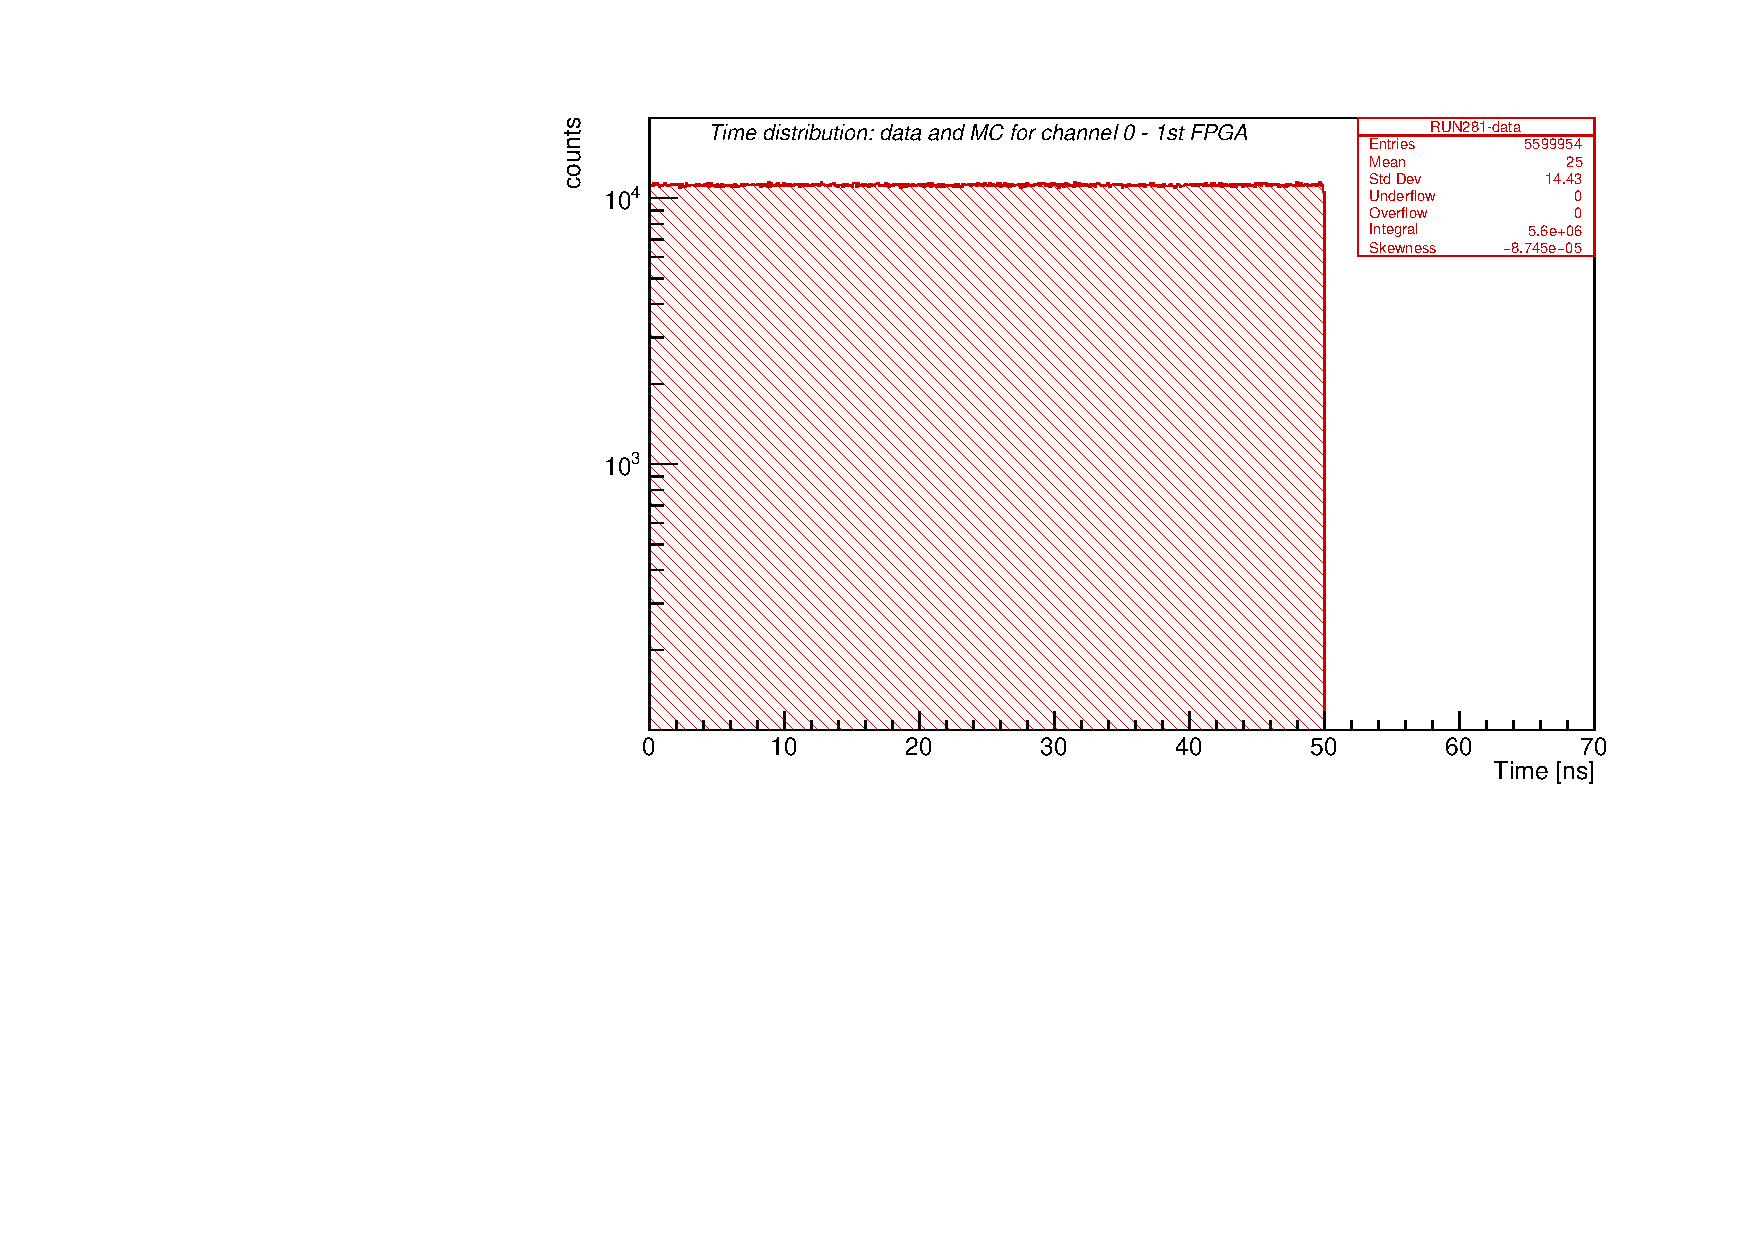
\includegraphics[width=0.5\textwidth]{figures/pdf/figure_00007_timedistr_roc_simulation_ch0_281}
      % }
    };
    \node[anchor=south west,inner sep=0] at (10,0.) {
      % \node[shift={(0 cm,0.cm)},inner sep=0,rotate={90}] at (0,0) {}
      % \makebox[\textwidth][c] {
      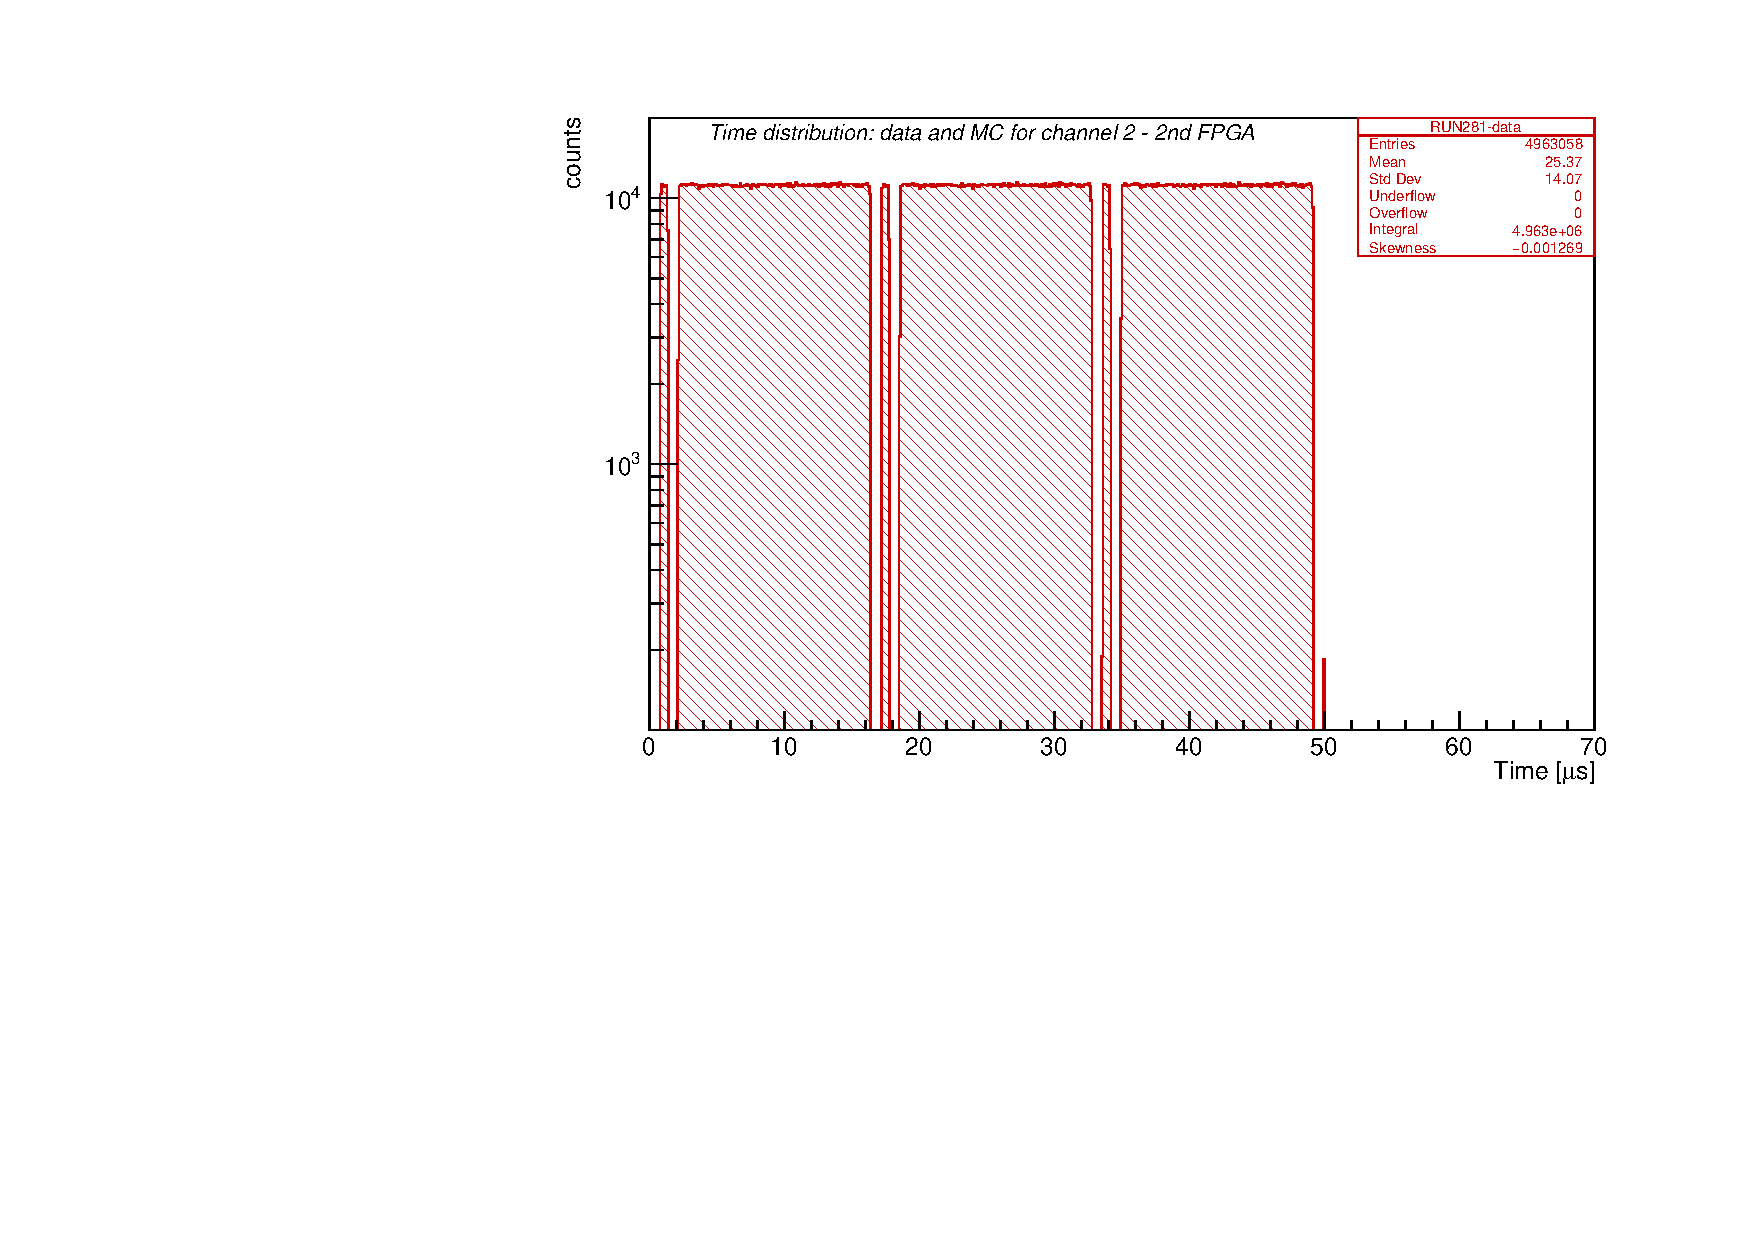
\includegraphics[width=0.5\textwidth]{figures/pdf/figure_00003_timedistr_roc_simulation_ch2_281}
      % }
    };
  \end{tikzpicture}
  \caption{
    \label{fig:1}
    right: channel 0 (first FPGA) time distribution of hits, left: channel 2 (second FPGA) time distribution of hits.
  }
\end{figure}
These distributions are easier to understand by looking at the occupancy plot in Fig.\ref{fig:2}. Channel ordering in this plot corresponds to the readout order.
This revealed a non uniform distribution. We compared with the Monte Carlo occupancy.
\begin{figure}[!h]
\centering
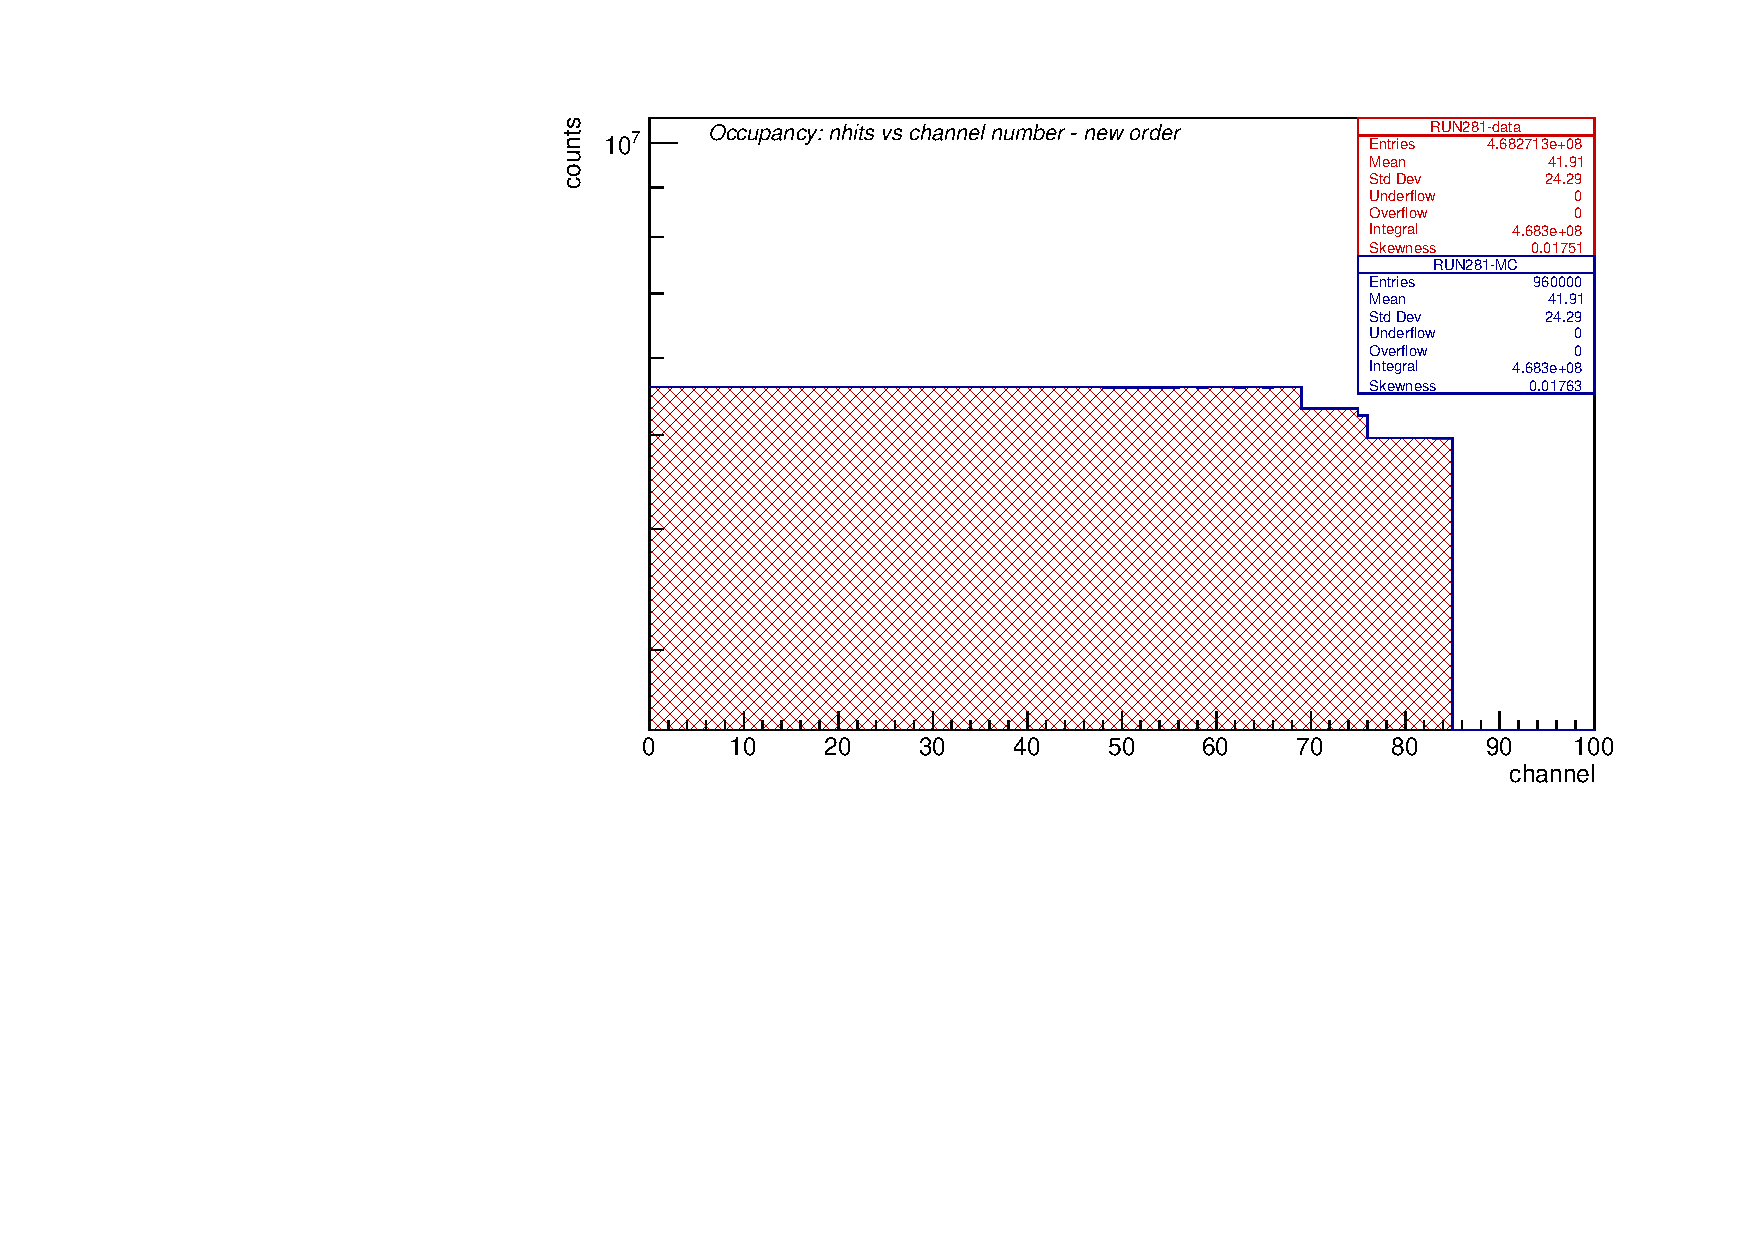
\includegraphics[width =0.8\textwidth]{figures/pdf/figure_00004_nhitsvschannel_roc_simulation_281}
\caption{Occupancy: number of hits versus channel. The ordering of channels adheres to the sequence prescribed by the Monte Carlo simulation.}
\label{fig:2}
\end{figure}
As we can see in the number of hits histogram ???, there could be 3 or 4 hits. 
The first 68 channels are the ones with 4 hits in the first FPGA and three in the second FPGA. The second plateau extending from 68 to 75 are the channels with 3 hits in the first FPGA and 4 hits in the second one. There is a big step at the end of this plateau, because if we count the number of hits in the first FPGA we get 144, so in the second FPGA we have 111 hits in total. 111 is not divisible by 4, so the first 27 channels in the second FPGA will have 4 hits and the last one will have 3 hits only. Last plateau consists of 3 hits from the first FPGA and 3 hits from the second FPGA.
Coming back to Fig.\ref{fig:1}, some channels are always readout and some others no, as we explained in the introduction the ROC hit buffer gets filled up and only the first 255 hits are read out. This results in uniform time distribution for the first channels readout and in a non unform time distribution for the last readout channels, depending on $T_{gen}$ and $T_{EW}$. The deeps in channel 2 are defined by the differences between the two pulsers. 





\subsection{Number of hits}
 Fig. \ref{fig:3} shows that we are reading out 255 hits as expected.
\begin{figure}[!h]
\centering
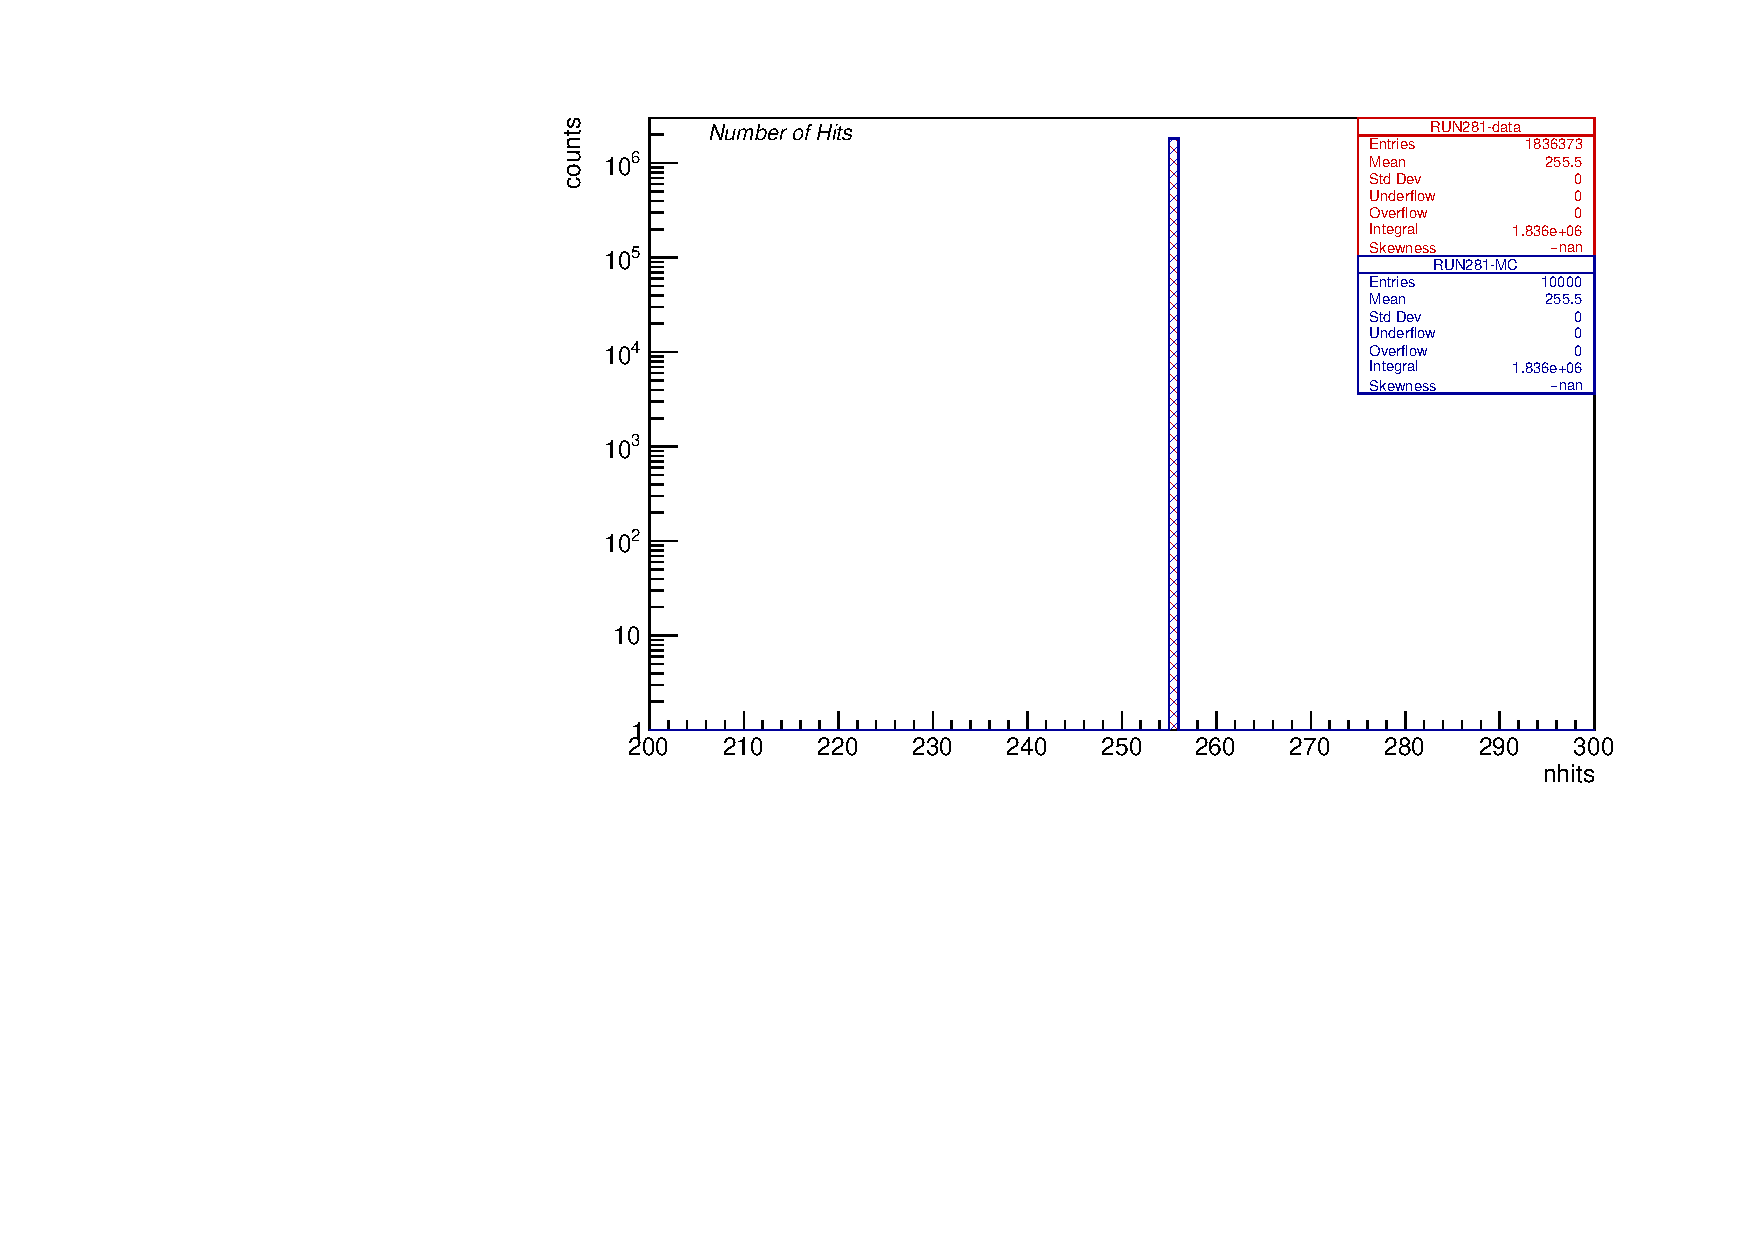
\includegraphics[width =0.8\textwidth]{figures/pdf/figure_00008_nhits_281}
\caption{Number of hits distribution.}
\label{fig:3}
\end{figure}


%%% Local Variables:
%%% mode: latex
%%% TeX-master: t
%%% End:
